\chapter*{Teoretisk genomgång}
\refstepcounter{chapter}

\section{Kaosteori}

Kaosteori är ett tvärvetenskapligt forskningsområde område som fokuserar på att studera mönster hos deterministiska system som är extremt känsliga till begynnelsevillkor \cite{britannica_chaos_theory_2025}. Med detta menas att, om inte exakt samma 

\section{Lagrange-mekanik}

För att lösa mer komplexa problem, som exempelvis dubbelpendeln, är det oftare lättare att använda Lagrange-mekanik för att beskriva dess rörelse. Även om det är teoretiskt sätt möjligt att beskriva en dubbelpendels rörelse med klassisk newtonsk mekanik, kan det fort bli mödosamt och onödigt krångligt. Lagrange-mekanik är egentligen bara en annan matematisk metod för att beskriva omvärlden, vilket i en viss typ av problem, blir betydligt lättare att lösa.

%För att lösa mer komplexa problem, som exempelvis dubbelpendeln, är det ofta lättare att använda Lagranges ekvationer för att beskriva dess rörelse. Även om det är teoretiskt möjligt att beskriva en dubbelpendels rörelse med klassisk newtonsk mekanik, kan det fort bli mödosamt och därmed används Lagranges ekvationer istället.

% En beskrivning av ett system med Lagranges ekvationer består oftast av the Lagrangian $\Lagr$ \cite{book:classical_mechanics:Morin2007}, där $T$ och $V$ är systemets kinetiska respektive lägesenergi, se ekvation (\ref{eq:Lagr}).
% \begin{equation} %% todo: varför är det [2] på referensen?
%     \Lagr = T - V
%     \label{eq:Lagr}
% \end{equation}
% Sedan ger Euler-Lagrange ekvationen (\ref{eq:euler_lagrange_equation}) att den ekvation som uppfyller (\ref{eq:Lagr}) är den ekvation som beskriver systemets rörelse \cite{book:classical_mechanics:Morin2007}.
% \begin{equation}
%     \frac{d}{dt}\left( \frac{\partial \Lagr}{\partial \dot{q_{i}}} \right) - \frac{\partial \Lagr}{\partial q_{i}} = 0,
%     \label{eq:euler_lagrange_equation}
% \end{equation}
% för varje $i = 1,2,3,\ldots$.

\subsection{Principen om minsta verkan}

Lagrange-mekanik bygger sin grund på \emph{principen om minsta verkan}, eller ibland även kallad \emph{principen om stationär verkan} \cite{Manton2013PrincipleLeastAction}. Denna princip säger därmed att ett objekt kommer alltid att sträva efter att färdas den väg som minimerar den fysikaliska \emph{verkan} \cite[s.2]{Manton2013PrincipleLeastAction}. Detta är så fysikaliskt grundläggande, att nästan all fysik kan härledas ur detta grundläggande antagande \cite{Manton2013PrincipleLeastAction}. Givet att vi har ett objekt $Q$ som rör sig längs $x(t)$, där $Q$ har startpunkten $x(t_1)$ och slutpunkten $x(t_2)$, samt att $T(t)$ och $V(t)$ är objektets rörelse respektive kinetiska energi, definieras verkan $S$ inom tidsintervallet $t_1\leq t \leq t_2$ som \cite[s.10]{Manton2013PrincipleLeastAction}:
\begin{equation} 
    S = \int_{t_1}^{t_2}\left(T(t)-V(t)\right)dt. \label{eq:action_definition}
\end{equation} 
Denna storhet har enheten [Js] och har dimensionerna (Energi $\times$ Tid) \cite[s.221]{book:classical_mechanics:Morin2007}. Själva differensen $T(t) - V(t)$ visar sig vara så relevant inom fysiken, att den har fått namnet 'the Lagrangian' och brukar betecknas $\Lagr$ \cite[s.218]{book:classical_mechanics:Morin2007}, det vill säga
\footnote{Varför $\Lagr = T(t) - V(t)$ är så viktigt i (\ref{eq:action_definition}) kan tyckas konstigt. Varför ska \emph{differensen} av kinetiska och potentiella energin spela någon roll? }:
\begin{equation} %% todo: varför är det [2] på referensen?
    \Lagr = T - V
    \label{eq:Lagr}
\end{equation}
Principen om minsta verkan säger att fysikens lagar strävar efter att förminska (\ref{eq:action_definition})\footnote{Egentligen, rent matematiskt, strävar verkan $S$ att hitta ett stationärt värde av $S$, det vill säga en lokal extrem- eller terrasspunkt till grafen av $S$. Detta är anledningen varför principen även kallas för \emph{principen om stationär verkan} \cite[s.222]{book:classical_mechanics:Morin2007}.}.

För att bestämma ett objekts väg som minimerar verkan $S$ används \emph{Euler-Lagrange ekvationen} \cite[s. 222]{book:classical_mechanics:Morin2007} se ekvation (\ref{eq:euler_lagrange_equation}). I ekvation (\ref{eq:euler_lagrange_equation}) är $i = 1,2,3,\ldots$, och normalt sätt betecknar de olika koordinataxlarna i systemet. Härledning av (\ref{eq:euler_lagrange_equation}) ges i appendix A. %% TODO, härledning av euler-lagrange ekvationen
\begin{equation}
    \frac{d}{dt}\left( \frac{\partial \Lagr}{\partial \dot{q_{i}}} \right) - \frac{\partial \Lagr}{\partial q_{i}} = 0,
    \label{eq:euler_lagrange_equation}
\end{equation}

%\subsubsection{Pedagogiskt exempel på tillämpning av Lagrange-mekanik}
%För att ge ett exempel på hur ekvation (\ref{eq:euler_lagrange_equation}) kan användas rent fysikaliskt\footnote{Hos många studenter kan det till en början kännas 'udda' varför (\ref{eq:Lagr}) och (\ref{eq:euler_lagrange_equation}) ens är relevanta. Därför tas detta exempel med, för att ge en viss intuition till att (\ref{eq:euler_lagrange_equation}) funkar.}, tas ett exempel på en boll med massan $m$. Om vi släpper bollen från vila, och låter den falla fritt (utan något luftmotstånd), kommer den ha fallit höjden $h$ under 1 sekund. Vi vet enligt de välkända kinematiska formlerna \cite{formelsamling} att $h=\frac{gt^2}{2}$, dvs bollen kommer att ha färdats $\frac{g}{2}$ m efter 1 sekund.  

% Verkan är en fysikalisk storhet som beskriver summan av , där om vi har ett objekt som rör sig mellan två punkter $x(t_1)$ och $x(t_2)$ inom tidsintervallet $(t_2 - t_1)$, så definieras verkan $S$ som \cite[s.10]{Manton2013PrincipleLeastAction}:
% \begin{equation} 
%     S = \int_{t_1}^{t_2}\left(T(t)-V(t)\right)dt. \label{eq:action_definition}
% \end{equation} 



% Det kan kännas spontant udda varför ekvationerna (\ref{eq:Lagr}) och (\ref{eq:euler_lagrange_equation}) ens är relevanta. Dessa ekvationer är dock en konsekvens av \emph{principen om minsta verkan}, vilket säger att ett objekt kommer alltid sträva efter att färdas den väg som minimerar den fysikaliska verkan \cite[s.2]{Manton2013PrincipleLeastAction}. Verkan är en fysikalisk storhet, där om vi har ett objekt som rör sig mellan två punkter $x(t_1)$ och $x(t_2)$ inom tidsintervallet $(t_2 - t_1)$, så definieras verkan $S$ som \cite[s.10]{Manton2013PrincipleLeastAction}:
% \begin{equation} 
%     S = \int_{t_1}^{t_2}\left(T(t)-V(t)\right)dt. \label{eq:action_definition}
% \end{equation} 
% Denna storhet har enheten [Js] och har dimensionerna (Energi $\times$ Tid). Det visar sig att \emph{principen om minsta verkan} är en princip som är minst lika fundamental som t.ex energiprincipen,


%Motivering och härledning av både (\ref{eq:Lagr}) och (\ref{eq:euler_lagrange_equation}) ges i appendix (TODO). %todo



\section{Dubbelpendeln}
Om två vanliga enkla pendlar är sammankopplade sägs de bilda en dubbelpendel, se figur \ref{fig:double_pendulum_schematic}. Den första pendeln består av en punktformig massa $m_1$ som är kopplad till en masslös pinne med längden $l_1$, vilket sitter i en friktionslös rotationspunkt $\nu$. Den andra pendeln består också av en punktformig massa $m_2$ som är kopplad till en masslös pinne med längden $l_2$. Denna andra pendeln har sin friktionslösa rotationspunkt tillkopplad i $m_1$. Den enda kraften som verkar på respektive massa är tyngdkraften.

Låt vinklarna $\theta_1$, $\theta_2$ vara vinklarna mellan den lodräta linjen från rotationspunkten och den faktiska positionen av pendeln, se figur \ref{fig:double_pendulum_schematic}. Vinklarna $\theta_1$ och $\theta_2$ är inte begränsade mellan $-\pi \leq \theta_{1,2} \leq \pi$, dvs de kan rotera fritt hur många varv som helst runt rotationspunkterna. Detta innebär självklart att respektive pendel inte kommer påverkas av varandra, t.ex att de inte kan slå in i varandra.

\begin{figure}[h!]
    \centering
    %\includegraphics[scale=1]{Double-pendulum-system.png}
    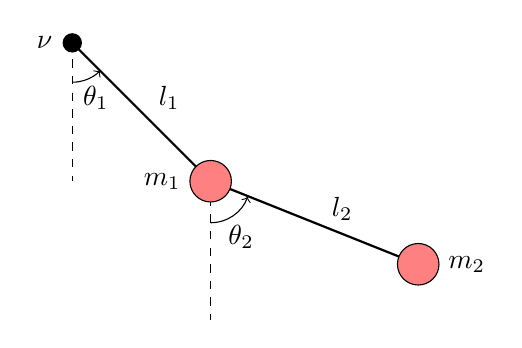
\begin{tikzpicture}

        \coordinate (O) at (0,0);

        \coordinate[yshift=-5pt,xshift=-5pt] (OL) at (O);

        \coordinate[yshift=-50pt] (OE) at (O);

        \coordinate[yshift=-50pt,xshift=50pt] (M1) at (O);

        \coordinate[yshift=-15] (MA) at (M1);

        \coordinate[yshift=-50pt] (ME) at (M1);

        \coordinate[yshift=-30pt,xshift=75pt] (M2) at (M1);

        \coordinate[yshift=-25,xshift=-25] (L) at (O);

        \draw[thick] (O) -- (M1) node[midway,xshift=10pt,yshift=5pt] {$l_1$} -- (M2) node[midway,xshift=10pt,yshift=5pt] {$l_2$};

        \draw[dashed] (O) -- (OE);

        \draw[dashed] (M1) -- (ME);


        \filldraw[color=black,fill=red!50] (M1) circle [radius=7.5pt];
        \filldraw[color=black,fill=red!50] (M2) circle [radius=7.5pt];

        \node[yshift=-20pt,xshift=8.5pt] at (O) {$\theta_1$};

        \node[yshift=-20pt,xshift=11pt] at (M1) {$\theta_2$};

        \node[xshift=-17.5pt] at (M1) {$m_1$};

        \node[xshift=17.5pt] at (M2) {$m_2$};

        %\draw[gray,ultra thick] (-3,0) -- (3,0);

        %\draw[->] (L) -- (OL);

        \node[xshift=-10pt] at (O) {$\nu$};

        % \draw[gray] (-3,0) -- (-2.5,0.35);

        % \draw[gray] (-2.5,0) -- (-2,0.35);

        % \draw[gray] (-2,0) -- (-1.5,0.35);

        % \draw[gray] (-1.5,0) -- (-1,0.35);

        % \draw[gray] (-1,0) -- (-0.5,0.35);

        % \draw[gray] (-0.5,0) -- (0,0.35);

        % \draw[gray] (0,0) -- (0.5,0.35);

        % \draw[gray] (0.5,0) -- (1,0.35);

        % \draw[gray] (1,0) -- (1.5,0.35);

        % \draw[gray] (1.5,0) -- (2,0.35);

        % \draw[gray] (2,0) -- (2.5,0.35);

        % \draw[gray] (2.5,0) -- (3,0.35);

        \fill[black] (O) circle [radius=3.5pt];

        \draw[->] (0,-0.5) arc (-90:-45:0.5);

        \draw[->] (MA) arc (-90:-20:0.5);
    \end{tikzpicture}
    \caption{Schematisk figur över en matematisk dubbelpendel.}
    \label{fig:double_pendulum_schematic}
\end{figure}


% Den första pendeln består av en masslös pinne med längden $l_1$ som sitter i en friktionslös vridpunkt $\nu$. Vid änden av pinnen sitter även en punktformig massa $m_1$. Därefter kopplas en till masslös pinne med längden $l_2$ på $m_1$ så att pinnen kan rotera friktionsfritt. Dessutom finns en till punktformig massa $m_2$ tillkopplad på änden av pinnen med längden $l_2$. Eftersom pinnarna är masslösa och all friktion kan försummas, kan denna uppställning av en dubbelpendel beskrivas som en matematisk dubbelpendel. Låt vinklarna $\theta_1$, $\theta_2$ vara vinklarna normalen taket och pinnarna till för respektive enkel pendel. Den resulterande accelerationen på massorna $m_1$, $m_2$ är tyngdaccelerationen $g$.

% Eftersom pinnarna är masslösa, massorna $m_1$, $m_2$ är punktformiga och all friktion försummas, sägs dubbelpendeln vara matematisk. Därmed kommer energin i hela system bevaras. 

% Den enda accelerationen som verkar på massorna $m_1$, $m_2$ antas vara tyngdaccelerationen $g$. 

% vara massorna för respektive enkla pendel, och låt $l_1$, $l_2$ vara längden av respektive pendels snöre/stav. För denna rapport kommer vi bara behandla matematiska pendlar, vilket innebär att massorna $m_1$, $m_2$ antas vara punktformiga och pendels snören anses vara masslösa. 


% Även om det är rent matematiskt möjligt att härleda formlerna som beskriver en dubbelpendels rörelse med klassisk mekanik, anses det



\subsection{Härledning av dubbelpendels rörelseekvationer} \label{sec:härledning_av_dubbelpendeln}

Härledningen utgår från figur \ref{fig:double_pendulum_schematic}, där dubbelpendeln ritats in i ett koordinatsystem där origo utgår från vridpunkten $\nu$. De punktformiga massorna $m_1$ och $m_2$ har koordinaterna $(x_1,y_1)$ respektive $(x_2,y_2)$.

Vi kan beskriva punkterna $x_1$, $x_2$, $y_1$ och $y_2$ genom trigonometri enligt:
\begin{align}
    x_1 & = l_1 \sin{\theta_1} \label{eq:x_1}                      \\
    y_1 & = -l_1\cos{\theta_1} \label{eq:y_1}                      \\
    x_2 & = l_1\sin{\theta_1} + l_2\sin{\theta_2} \label{eq:x_2}   \\
    y_2 & = -l_1\cos{\theta_1} - l_2\cos{\theta_2}. \label{eq:y_2}
\end{align}

Eftersom tidsderivatan av sträcka/position är hastighet, kan vi få hastigheterna $\dot{x}_1$, $\dot{y}_1$, $\dot{x}_2$ och $\dot{y}_2$ enligt:
\begin{align}
    \dot{x}_1 & = \dot{\theta}_1 l_1 \cos{\theta_1} \label{eq:x_1:dot}                   \\
    \dot{y}_1 & = \dot{\theta}_1 l_1 \sin{\theta_1} \label{eq:y_1:dot}                   \\
    \dot{x}_2 & = \dot{\theta}_1 l_1 \cos{\theta_1} + \dot{\theta}_2 l_2 \cos{\theta_2} \label{eq:x_2:dot}  \\
    \dot{y}_2 & = \dot{\theta}_1 l_1 \sin{\theta_1} + \dot{\theta}_2 l_2 \sin{\theta_2}. \label{eq:y_2:dot}
\end{align}

Vi kan därmed definiera dubbelpendelns potentiella energi $V$ som summan av den potentiella energin för respektive massa. Detta ger:
\begin{align}
    V                                              & = m_1gy_1 + m_2gy_2 \notag                                                       \\
    (\ref{eq:y_1}),\/ (\ref{eq:y_2}) \Rightarrow V & = -(m_1 + m_2)gl_1\cos{\theta_1} - m_2gl_2\cos{\theta_2}. \label{eq:V/potential_energy}
\end{align}

Vi kan också bestämma dubbelpendelns kinetiska energi $T$ enligt:
\begin{align}
    T   &= \frac{1}{2} m_1 v_{1}^{2} + \frac{1}{2}m_2v_2^2 \notag \\
        &= \frac{1}{2}m_1\left(\dot{x}_1^2 + \dot{y}_1^2\right) + \frac{1}{2}m_2\left(\dot{x}_2^2 + \dot{y}_2^2\right) \notag \\ %% TODO; motivera kanske varför v^2 = v_x^2 + v_y^2
    (\ref{eq:x_1:dot}) - (\ref{eq:y_2:dot}) \Rightarrow &= \frac{1}{2}m_1\left(\dot{\theta}_1^2 l_1^2 \cos^2{\theta_1} + \dot{\theta}_1^2 l_1^2 \sin^2{\theta_1}\right) + \frac{1}{2}m_2
    \left(
        \dot{\theta}_1^2 l_1^2 \cos^2{\theta_1}\right. \notag \\
        &\quad + 2\dot{\theta}_1\dot{\theta}_2l_1l_2\cos{\theta_1}\cos{\theta_2}
        + \dot{\theta}_2^2l_2^2\cos^2{\theta_2} \dot{\theta}_1^2l_1^2\sin^2{\theta_1} \notag \\
        &\quad + \left.2\dot{\theta}_1\dot{\theta}_2l_1l_2\sin{\theta_1}\sin{\theta_2} + \dot{\theta}_2^2l_2^2\sin^2{\theta_2}
    \right) \notag \\
    \Rightarrow &= \frac{1}{2}m_1\dot{\theta}_1^2l_1^2\left(\cos^2{\theta_1} + \sin^2{\theta_1}\right) + \frac{1}{2}m_2\left( \dot{\theta}_1^2l_1^2\left(\sin^2{\theta_1} + \cos^2{\theta_1}\right) \right. \notag \\
    &\quad + \left.\dot{\theta}_2^2l_2^2\left(\sin^2{\theta_2} + \cos^2{\theta_2}\right) 2\dot{\theta}_1\dot{\theta}_2l_1l_2\left(\cos{\theta_1}\cos{\theta_2} + \sin{\theta_1}\sin{\theta_2}\right)\right). \notag
\end{align}

Eftersom $\sin^2{\theta} + \cos^2{\theta} = 1$ och $\cos{\theta_1}\cos{\theta_2} + \sin{\theta_1}\sin{\theta_2} = \cos(\theta_1 - \theta_2)$ (trigonometriska ettan respektive subtraktionsformeln för cosinus) kan vi förenkla uttrycket till:

\begin{equation}
    T = \frac{1}{2}m_1\dot{\theta}_1^2l_1^2 + \frac{1}{2}m_2\left(\dot{\theta}_1^2l_1^2 + \dot{\theta}_2^2l_2 + 2\dot{\theta}_1\dot{\theta}_2l_1l_2\cos(\theta_1-\theta_2)\right). \label{eq:T/kinetic_energy_simplified}
\end{equation}

Nu när vi har uttryckt $V$ och $T$ som funktioner av $\theta_1$ och $\theta_2$, kan vi beräkna $\Lagr$. Enligt (\ref{eq:Lagr}), (\ref{eq:V/potential_energy}) och (\ref{eq:T/kinetic_energy_simplified}) får vi att:
\begin{align}
    \Lagr               &= T - V \notag \\
                        &= \frac{1}{2}m_1\dot{\theta}_1^2l_1^2 + \frac{1}{2}m_2\left(\dot{\theta}_1^2l_1^2 + \dot{\theta}_2^2l_2^2 + 2\dot{\theta}_1\dot{\theta}_2l_1l_2\cos(\theta_1-\theta_2)\right) \notag \\
                        &\quad - \left(-(m_1 + m_2)gl_1\cos{\theta_1} - m_2gl_2\cos{\theta_2}\right) \notag \\
    \Rightarrow \Lagr   &= \frac{1}{2}m_1\dot{\theta}_1^2l_1^2 + \frac{1}{2}m_2\left(\dot{\theta}_1^2l_1^2 + \dot                {\theta}_2^2l_2^2 + 2\dot{\theta}_1\dot{\theta}_2l_1l_2\cos(\theta_1-\theta_2)\right) \notag \\
                        &\quad + (m_1 + m_2)gl_1\cos{\theta_1} + m_2gl_2\cos{\theta_2}. \label{eq:Lagr_simplified}
\end{align}

\subsubsection{Tillämpning av Euler-Lagrange ekvationen}

Vi ska nu använda ekvation (\ref{eq:Lagr_simplified}) i Euler-Lagrange ekvationen (\ref{eq:euler_lagrange_equation}) för att lösa ut ekvationen som beskriver vinklarna $\theta_1$ och $\theta_2$ i dubbelpendeln. Vi beräknar för fallet för $q_i=\theta_1$.

Deriveringsregler för att bestämma $ \frac{\partial \Lagr}{\partial \dot{\theta}_1}$ och $\frac{d}{dt}\!\left(\frac{\partial \Lagr}{\partial \dot{\theta}_1}\right)$ ger:
\begin{align}
    \frac{\partial \Lagr}{\partial \dot{\theta}_1} &= m_1l_1^2\dot{\theta}_1+ m_2l_1^2\dot{\theta}_1 + m_2l_1l_2\dot{\theta}_2\cos(\theta_1-\theta_2) \notag \\
    \Rightarrow \frac{d}{dt}\left(\frac{\partial \Lagr}{\partial \dot{\theta}_1}\right) &= m_1l_1^2\ddot{\theta}_1 + m_2l_1^2\ddot{\theta}_1 + m_2l_1l_2\ddot{\theta}_2\cos(\theta_1-\theta_2) \notag\\
    &\quad - m_2l_1l_2\dot{\theta}_2\sin(\theta_1-\theta_2)(\dot{\theta}_1-\dot{\theta}_2) \notag \\
    \Rightarrow \frac{d}{dt}\left(\frac{\partial \Lagr}{\partial \dot{\theta}_1}\right) &= \left(m_1+m_2\right)l_1^2\ddot{\theta}_1 + m_2l_1l_2\ddot{\theta}_2\cos(\theta_1-\theta_2) \notag \\
    &\quad - m_2l_1l_2\dot{\theta}_1\dot{\theta}_2\sin(\theta_1-\theta_2) + m_2l_1l_2\dot{\theta}_2^2\sin(\theta_1-\theta_2). \label{eq:Lagr_time_derivative:respect_theta_1_dot}
\end{align}

Deriveringsregler för att bestämma $\frac{\partial \Lagr}{\partial \theta_1}$ ger:
\begin{align}
    \frac{\partial \Lagr}{\partial \theta_1} &= -m_2l_1l_2\dot{\theta}_1\dot{\theta}_2\sin(\theta_1-\theta_2) - \left(m_1 + m_2\right)gl_1\sin{\theta_1}. \label{eq:Lagr_derivative:repsect_theta_1}
\end{align}

Insättning av (\ref{eq:Lagr_time_derivative:respect_theta_1_dot}) och (\ref{eq:Lagr_derivative:repsect_theta_1}) i (\ref{eq:euler_lagrange_equation}) ger att:
\begin{align}
    0 &=\left(m_1+m_2\right)l_1^2\ddot{\theta}_1 + m_2l_1l_2\ddot{\theta}_2\cos(\theta_1-\theta_2)
    - m_2l_1l_2\dot{\theta}_1\dot{\theta}_2\sin(\theta_1-\theta_2) \notag \\
    &\quad + m_2l_1l_2\dot{\theta}_2^2\sin(\theta_1-\theta_2) + m_2l_1l_2\dot{\theta}_1\dot{\theta}_2\sin(\theta_1-\theta_2) + \left(m_1 + m_2\right)gl_1\sin{\theta_1} \notag\\
    \Leftrightarrow 0 &= \left(m_1+m_2\right)l_1\ddot{\theta}_1 + m_2l_2\ddot{\theta}_2\cos(\theta_1-\theta_2)
    + m_2l_2\dot{\theta}_2^2\sin(\theta_1-\theta_2) \notag \\
    &\quad + \left(m_1 + m_2\right)g\sin{\theta_1}. \label{eq:theta_1_solution}
\end{align}

Därmed är (\ref{eq:theta_1_solution}) ekvationen som beskriver vinkeln $\theta_1$ i dubbelpendeln. Nu ska vi istället lösa Euler-Lagrange ekvationen (\ref{eq:euler_lagrange_equation}) fast för $q_i = \theta_2$.

Deriveringsregler för att bestämma $ \frac{\partial \Lagr}{\partial \dot{\theta}_2}$ och $\frac{d}{dt}\!\left(\frac{\partial \Lagr}{\partial \dot{\theta}_2}\right)$ ger:
\begin{align}
    \frac{\partial \Lagr}{\partial \dot{\theta}_2} &= m_2l_2^2\dot{\theta}_2 + m_2l_1l_2\dot{\theta}_1\cos(\theta_1 - \theta_2) \notag\\
    \Rightarrow \frac{d}{dt}\left(\frac{\partial \Lagr}{\partial \dot{\theta}_2}\right) &= m_2l_2^2\ddot{\theta}_2 + m_2l_1l_2\left(\ddot{\theta}_1\cos(\theta_1-\theta_2) - \dot{\theta}_1\sin(\theta_1 - \theta_2)(\dot{\theta}_1 - \dot{\theta}_2)\right) \notag \\
    \Rightarrow \frac{d}{dt}\left(\frac{\partial \Lagr}{\partial \dot{\theta}_2}\right) &= m_2l_2^2\ddot{\theta}_2 + m_2l_1l_2\ddot{\theta}_1\cos(\theta_1-\theta_2) - m_2l_1l_2\dot{\theta}_1^2\sin(\theta_1-\theta_2) \notag \\
    &\quad + m_2l_1l_2\dot{\theta}_1\dot{\theta}_2\sin(\theta_1 - \theta_2). \label{eq:Lagr_time_derivative:respect_theta_2_dot}
\end{align}

Deriveringsregler för att bestämma $\frac{\partial \Lagr}{\partial \theta_2}$ ger:
\begin{align}
    \frac{\partial \Lagr}{\partial \theta_2} &= m_2l_1l_2\dot{\theta}_1\dot{\theta}_2\sin(\theta_1-\theta_2) - m_2gl_2\sin{\theta_2}.  \label{eq:Lagr_derivative:repsect_theta_2}
\end{align}

Insättning av (\ref{eq:Lagr_time_derivative:respect_theta_2_dot}) och (\ref{eq:Lagr_derivative:repsect_theta_2}) i (\ref{eq:euler_lagrange_equation}) ger:
\begin{align}
    0 &= m_2l_2^2\ddot{\theta}_2 + m_2l_1l_2\ddot{\theta}_1\cos(\theta_1 - \theta_2) - m_2l_1l_2\dot{\theta}_1^2\sin(\theta_1-\theta_2) \notag \\
    &\quad + m_2l_1l_2\dot{\theta_1}\dot{\theta}_2\sin(\theta_1 - \theta_2) - m_2l_1l_2\dot{\theta}_1\dot{\theta}_2\sin(\theta_1-\theta_2) + m_2gl_2\sin{\theta_2} \notag \\
    \Leftrightarrow 0 &= m_2l_2\ddot{\theta}_2 + m_2l_1\ddot{\theta}_1\cos(\theta_1 - \theta_2) - m_2l_1\dot{\theta}_1^2\sin(\theta_1 - \theta_2) + m_2g\sin{\theta_2}. \label{eq:theta_2_solution}
\end{align}

Detta innebär att (\ref{eq:theta_2_solution}) är den ekvation som beskriver vinkeln $\theta_2$ i dubbelpendeln. Därmed har vi nu funnit våra två ekvationer som enligt Euler-Lagrange ekvationen (\ref{eq:euler_lagrange_equation}) beskriver dubbelpendelns rörelse, se ekvationssystemet (\ref{eq:equations_of_motion}):
\begin{equation} \begin{cases}
        0 &= \left(m_1+m_2\right)l_1\ddot{\theta}_1 + m_2l_2\ddot{\theta}_2\cos(\theta_1-\theta_2)
        + m_2l_2\dot{\theta}_2^2\sin(\theta_1-\theta_2) \\
        &\quad + \left(m_1 + m_2\right)g\sin{\theta_1}. \\
        0 &= m_2l_2\ddot{\theta}_2 + m_2l_1\ddot{\theta}_1\cos(\theta_1 - \theta_2) - m_2l_1\dot{\theta}_1^2\sin(\theta_1 - \theta_2) + m_2g\sin{\theta_2}. \label{eq:equations_of_motion}
\end{cases} \end{equation}

Ekvationssystemet i (\ref{eq:equations_of_motion}) går inte att lösa analytiskt, utan måste skrivas om för att få (\ref{eq:equations_of_motion}) till en ordinär första ordningens differentialekvation (ODE). Detta kan göras genom att införa nya beteckningar för vinkelhastigheterna $\omega_1$ och $\omega_2$, dvs $\omega_1 = \dot{\theta_1}$ och $\omega_2 = \dot{\theta_2}$. Därmed kan (\ref{eq:equations_of_motion}) skrivas om enligt ekvationssystemet (\ref{eq:equations_of_motion_with_omega}). 

\begin{equation}
    \begin{cases}
        \dot{\theta}_1 = \omega_1  \\
        \dot{\theta}_2 = \omega_2 \\
        \dot{\omega}_1 = - \frac{m_2l_2\dot{\omega}_2^2\cos(\theta_1 - \theta_2) + m_1l_2\omega_2^2\sin(\theta_1-\theta_2) + (m_1+m_2)g\sin{\theta_1}}{(m_1+m_2)l_1} \\
        \dot{\omega}_2 = - \frac{m_2l_1\dot{\omega}_1\cos(\theta_1-\theta_2) - m_2l_1\omega^2_1\sin(\theta_1 - \theta_2 + m_2g\sin{\theta_2})}{m_2l_2} \label{eq:equations_of_motion_with_omega}
    \end{cases}
\end{equation}

Däremot har (\ref{eq:equations_of_motion_with_omega}) problemet att de tredje och fjärde ekvationerna är sammankopplade (på engelska, 'coupled'). Dessa två måste separeras för att kunna lösas numeriskt.  

\section{Numerisk metod för att lösa differentialekvationer}

Differentialekvationerna i (\ref{eq:equations_of_motion}) är icke-linjära och av andra ordningen, vilket gör de omöjligt att lösa rent analystiskt. Därmed måste ekvationerna lösas numeriskt, vilket kan göras med \emph{Runge-Kuttametoden}. Denna metod\footnote{Egentligen är Runge-Kuttametoden är en familj av metoder, då den innefattar ett flertal metoder, bland annat Eulers stegmetod. Däremot brukas RK4-metoden menas med ''Runge-Kuttametoden'', vilket är den vi kommer att använda här. För vidare förklaring, se \cite{Runge-Kutta_method/Butcher2008}. }, utvecklat och namngivet av de tyska matematikerna Carl Runge och Martin Willhelm Kutta, är en kraftfull metod för att lösa ordinära differentialekvationer (ODE:s) \cite[s. 93]{Runge-Kutta_method/Butcher2008}. 

Runge-Kuttametoden ger oss en metod att lösa ekvationer på formen $x' = f(t,x)$, där $x(t)$ är den okända funktionen. Metoden bygger på att approximera lösningen stegvis med ett litet $h$, men istället för att bara beräkna nuvarande lutningen (det som sker i Eulers metod), så beräknas flera mellanliggande lutningar där ett viktad medelvärde istället dras. 


\subsection{Behandling av dubbelpendelns rörelseekvationer för att möjliggöra RK4-metoden}


\subsection{Allmänna definitionen av RK4-metoden}

Låt $\mathbf{x}$ vara en tillståndsvektor sådan att $\mathbf{x} = [x_1, x_2, \ldots, x_n]^T$, $\mathbf{x}' = \frac{d\mathbf{x}}{dt}$ och låt $\mathbf{f} = [f_1, f_2, \ldots, f_n]^T$. Dessutom har vi begynnelsevärdet TODO Vi vill beräkna värdet av tillståndsvektorn $\bf{x}$ över tidsintervallet $[t_0, t]$ med steglängden $h$. Givet att $\bf{x'} = f(t,x)$, så definieras nästa tillståndsvektor $\bf{x_{n+1}}$ enligt: 
\begin{equation}
    \mathbf{x}_{n+1} = x_n + \frac{h}{6}\left(\mathbf{K}_{1n} + 2\mathbf{K}_{2n} + 2\mathbf{K}_{3n} + \mathbf{K}_{4n}\right),
\end{equation}
\begin{equation}
    t_{n+1} = t_n + h,
\end{equation}
där värdena av $\mathbf{K}_{1n}, \mathbf{K}_{2n}, \mathbf{K}_{3n}$ och $\mathbf{K}_{4n}$ är definierade sådan att:
\begin{align}
    \mathbf{K}_{1n} &= \mathbf{f}(t,\mathbf{x}_n) \\
    \mathbf{K}_{2n} &= \mathbf{f}\left(t + \frac{h}{2}, \mathbf{x}_n + \frac{h}{2}\mathbf{K}_{1n}\right) \\
    \mathbf{K}_{3n} &= \mathbf{f}\left(t + \frac{h}{2}, \mathbf{x}_n + \frac{h}{2}\mathbf{K}_{2n}\right) \\
    \mathbf{K}_{4n} &= \mathbf{f}\left(t + h, \mathbf{x}_n + h\mathbf{K}_{3n}\right)
\end{align}


\footnote{Definitionen av RK4-metoden är hämtat från \cite{Allard2015DoublePendulum/Runge-Kutta-definition}}